\documentclass[twoside]{book}

% Packages required by doxygen
\usepackage{fixltx2e}
\usepackage{calc}
\usepackage{doxygen}
\usepackage[export]{adjustbox} % also loads graphicx
\usepackage{graphicx}
\usepackage[utf8]{inputenc}
\usepackage{makeidx}
\usepackage{multicol}
\usepackage{multirow}
\PassOptionsToPackage{warn}{textcomp}
\usepackage{textcomp}
\usepackage[nointegrals]{wasysym}
\usepackage[table]{xcolor}

% Font selection
\usepackage[T1]{fontenc}
\usepackage[scaled=.90]{helvet}
\usepackage{courier}
\usepackage{amssymb}
\usepackage{sectsty}
\renewcommand{\familydefault}{\sfdefault}
\allsectionsfont{%
  \fontseries{bc}\selectfont%
  \color{darkgray}%
}
\renewcommand{\DoxyLabelFont}{%
  \fontseries{bc}\selectfont%
  \color{darkgray}%
}
\newcommand{\+}{\discretionary{\mbox{\scriptsize$\hookleftarrow$}}{}{}}

% Page & text layout
\usepackage{geometry}
\geometry{%
  a4paper,%
  top=2.5cm,%
  bottom=2.5cm,%
  left=2.5cm,%
  right=2.5cm%
}
\tolerance=750
\hfuzz=15pt
\hbadness=750
\setlength{\emergencystretch}{15pt}
\setlength{\parindent}{0cm}
\setlength{\parskip}{3ex plus 2ex minus 2ex}
\makeatletter
\renewcommand{\paragraph}{%
  \@startsection{paragraph}{4}{0ex}{-1.0ex}{1.0ex}{%
    \normalfont\normalsize\bfseries\SS@parafont%
  }%
}
\renewcommand{\subparagraph}{%
  \@startsection{subparagraph}{5}{0ex}{-1.0ex}{1.0ex}{%
    \normalfont\normalsize\bfseries\SS@subparafont%
  }%
}
\makeatother

% Headers & footers
\usepackage{fancyhdr}
\pagestyle{fancyplain}
\fancyhead[LE]{\fancyplain{}{\bfseries\thepage}}
\fancyhead[CE]{\fancyplain{}{}}
\fancyhead[RE]{\fancyplain{}{\bfseries\leftmark}}
\fancyhead[LO]{\fancyplain{}{\bfseries\rightmark}}
\fancyhead[CO]{\fancyplain{}{}}
\fancyhead[RO]{\fancyplain{}{\bfseries\thepage}}
\fancyfoot[LE]{\fancyplain{}{}}
\fancyfoot[CE]{\fancyplain{}{}}
\fancyfoot[RE]{\fancyplain{}{\bfseries\scriptsize Generated by Doxygen }}
\fancyfoot[LO]{\fancyplain{}{\bfseries\scriptsize Generated by Doxygen }}
\fancyfoot[CO]{\fancyplain{}{}}
\fancyfoot[RO]{\fancyplain{}{}}
\renewcommand{\footrulewidth}{0.4pt}
\renewcommand{\chaptermark}[1]{%
  \markboth{#1}{}%
}
\renewcommand{\sectionmark}[1]{%
  \markright{\thesection\ #1}%
}

% Indices & bibliography
\usepackage{natbib}
\usepackage[titles]{tocloft}
\setcounter{tocdepth}{3}
\setcounter{secnumdepth}{5}
\makeindex

% Hyperlinks (required, but should be loaded last)
\usepackage{ifpdf}
\ifpdf
  \usepackage[pdftex,pagebackref=true]{hyperref}
\else
  \usepackage[ps2pdf,pagebackref=true]{hyperref}
\fi
\hypersetup{%
  colorlinks=true,%
  linkcolor=blue,%
  citecolor=blue,%
  unicode%
}

% Custom commands
\newcommand{\clearemptydoublepage}{%
  \newpage{\pagestyle{empty}\cleardoublepage}%
}

\usepackage{caption}
\captionsetup{labelsep=space,justification=centering,font={bf},singlelinecheck=off,skip=4pt,position=top}

%===== C O N T E N T S =====

\begin{document}

% Titlepage & ToC
\hypersetup{pageanchor=false,
             bookmarksnumbered=true,
             pdfencoding=unicode
            }
\pagenumbering{roman}
\begin{titlepage}
\vspace*{7cm}
\begin{center}%
{\Large neuralnetwork }\\
\vspace*{1cm}
{\large Generated by Doxygen 1.8.11}\\
\end{center}
\end{titlepage}
\clearemptydoublepage
\tableofcontents
\clearemptydoublepage
\pagenumbering{arabic}
\hypersetup{pageanchor=true}

%--- Begin generated contents ---
\chapter{Class Index}
\section{Class List}
Here are the classes, structs, unions and interfaces with brief descriptions\+:\begin{DoxyCompactList}
\item\contentsline{section}{\hyperlink{structDataset}{Dataset} }{\pageref{structDataset}}{}
\item\contentsline{section}{\hyperlink{structDatum}{Datum} }{\pageref{structDatum}}{}
\item\contentsline{section}{\hyperlink{structLossFunction}{Loss\+Function} }{\pageref{structLossFunction}}{}
\item\contentsline{section}{\hyperlink{structNeuralNet}{Neural\+Net} }{\pageref{structNeuralNet}}{}
\item\contentsline{section}{\hyperlink{structOptimizer}{Optimizer} }{\pageref{structOptimizer}}{}
\item\contentsline{section}{\hyperlink{structTensor}{Tensor} }{\pageref{structTensor}}{}
\end{DoxyCompactList}

\chapter{Class Documentation}
\hypertarget{structDataset}{}\section{Dataset Struct Reference}
\label{structDataset}\index{Dataset@{Dataset}}


Collaboration diagram for Dataset\+:
\nopagebreak
\begin{figure}[H]
\begin{center}
\leavevmode
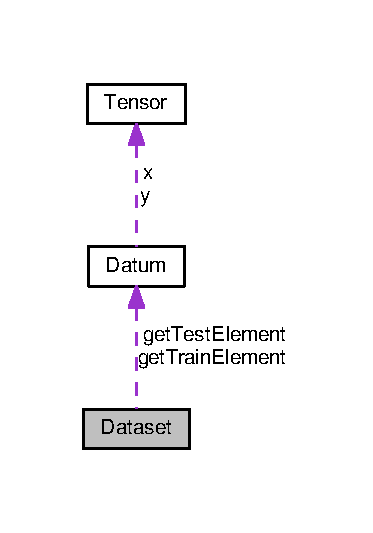
\includegraphics[width=179pt]{structDataset__coll__graph}
\end{center}
\end{figure}
\subsection*{Public Attributes}
\begin{DoxyCompactItemize}
\item 
size\+\_\+t {\bfseries train\+Elements}\hypertarget{structDataset_a0eb16d341ffee1ffd7bf831d4676251f}{}\label{structDataset_a0eb16d341ffee1ffd7bf831d4676251f}

\item 
\hyperlink{structDatum}{Datum}($\ast$ {\bfseries get\+Train\+Element} )(size\+\_\+t)\hypertarget{structDataset_ad56275ffce4161b71f63b319e92da258}{}\label{structDataset_ad56275ffce4161b71f63b319e92da258}

\item 
size\+\_\+t {\bfseries test\+Elements}\hypertarget{structDataset_aeef72e19c9615218257d0f243a0cee0c}{}\label{structDataset_aeef72e19c9615218257d0f243a0cee0c}

\item 
\hyperlink{structDatum}{Datum}($\ast$ {\bfseries get\+Test\+Element} )(size\+\_\+t)\hypertarget{structDataset_a76a75f489d541ab4dba3fd3c9e201b27}{}\label{structDataset_a76a75f489d541ab4dba3fd3c9e201b27}

\item 
void($\ast$ {\bfseries shuffle} )()\hypertarget{structDataset_a1d4de9bcd0037a298f992aee2864fb6d}{}\label{structDataset_a1d4de9bcd0037a298f992aee2864fb6d}

\end{DoxyCompactItemize}


The documentation for this struct was generated from the following file\+:\begin{DoxyCompactItemize}
\item 
dataset.\+h\end{DoxyCompactItemize}

\hypertarget{structDatum}{}\section{Datum Struct Reference}
\label{structDatum}\index{Datum@{Datum}}


Collaboration diagram for Datum\+:
\nopagebreak
\begin{figure}[H]
\begin{center}
\leavevmode
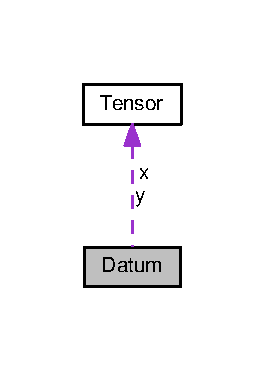
\includegraphics[width=127pt]{structDatum__coll__graph}
\end{center}
\end{figure}
\subsection*{Public Attributes}
\begin{DoxyCompactItemize}
\item 
\hyperlink{structTensor}{Tensor} $\ast$ {\bfseries x}\hypertarget{structDatum_a4122bf5e7a2709d3dc50185198e5852e}{}\label{structDatum_a4122bf5e7a2709d3dc50185198e5852e}

\item 
\hyperlink{structTensor}{Tensor} $\ast$ {\bfseries y}\hypertarget{structDatum_aeb7df532867627568e927b47c9ea9dd0}{}\label{structDatum_aeb7df532867627568e927b47c9ea9dd0}

\end{DoxyCompactItemize}


The documentation for this struct was generated from the following file\+:\begin{DoxyCompactItemize}
\item 
dataset.\+h\end{DoxyCompactItemize}

\hypertarget{structLossFunction}{}\section{Loss\+Function Struct Reference}
\label{structLossFunction}\index{Loss\+Function@{Loss\+Function}}
\subsection*{Public Attributes}
\begin{DoxyCompactItemize}
\item 
float($\ast$ {\bfseries loss} )(\hyperlink{structTensor}{Tensor} $\ast$, \hyperlink{structTensor}{Tensor} $\ast$)\hypertarget{structLossFunction_ac9674bcf59bf0721d777958fdd727928}{}\label{structLossFunction_ac9674bcf59bf0721d777958fdd727928}

\item 
void($\ast$ {\bfseries loss\+Derivative} )(\hyperlink{structTensor}{Tensor} $\ast$, \hyperlink{structTensor}{Tensor} $\ast$, \hyperlink{structTensor}{Tensor} $\ast$)\hypertarget{structLossFunction_adaa799b91da3c341091e6f57a1f10ded}{}\label{structLossFunction_adaa799b91da3c341091e6f57a1f10ded}

\item 
bool($\ast$ {\bfseries correct} )(\hyperlink{structTensor}{Tensor} $\ast$, \hyperlink{structTensor}{Tensor} $\ast$)\hypertarget{structLossFunction_a561e98d47acdeb0f07316ea47cc8b576}{}\label{structLossFunction_a561e98d47acdeb0f07316ea47cc8b576}

\end{DoxyCompactItemize}


The documentation for this struct was generated from the following file\+:\begin{DoxyCompactItemize}
\item 
loss\+\_\+functions.\+h\end{DoxyCompactItemize}

\hypertarget{structNeuralNet}{}\section{Neural\+Net Struct Reference}
\label{structNeuralNet}\index{Neural\+Net@{Neural\+Net}}


Collaboration diagram for Neural\+Net\+:
\nopagebreak
\begin{figure}[H]
\begin{center}
\leavevmode
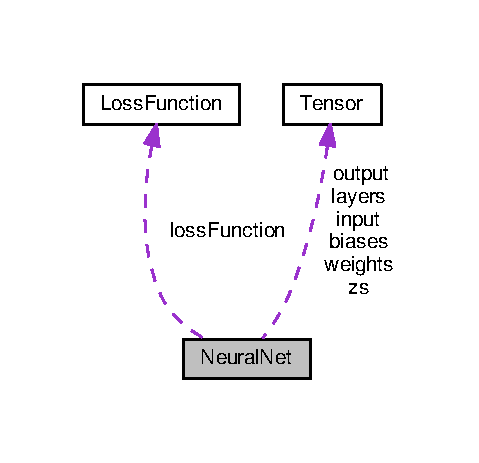
\includegraphics[width=230pt]{structNeuralNet__coll__graph}
\end{center}
\end{figure}
\subsection*{Public Attributes}
\begin{DoxyCompactItemize}
\item 
unsigned int {\bfseries depth}\hypertarget{structNeuralNet_ae3b433e9ccb78a471e8ccde61e82eed4}{}\label{structNeuralNet_ae3b433e9ccb78a471e8ccde61e82eed4}

\item 
unsigned int $\ast$ {\bfseries shape}\hypertarget{structNeuralNet_a1b4f8d7fccd76ed311b6daf17ac9b422}{}\label{structNeuralNet_a1b4f8d7fccd76ed311b6daf17ac9b422}

\item 
bool {\bfseries train}\hypertarget{structNeuralNet_a98890c143f4cfe67fa53725e8fc8363d}{}\label{structNeuralNet_a98890c143f4cfe67fa53725e8fc8363d}

\item 
\hyperlink{structTensor}{Tensor} $\ast$ {\bfseries input}\hypertarget{structNeuralNet_a254652197189ea13a3dbc39c018a1cfe}{}\label{structNeuralNet_a254652197189ea13a3dbc39c018a1cfe}

\item 
\hyperlink{structTensor}{Tensor} $\ast$ {\bfseries output}\hypertarget{structNeuralNet_a4e4276eed10edea3c2131d7d8adf6ea7}{}\label{structNeuralNet_a4e4276eed10edea3c2131d7d8adf6ea7}

\item 
\hyperlink{structTensor}{Tensor} $\ast$$\ast$ {\bfseries layers}\hypertarget{structNeuralNet_a4e067fc722269cfa5cba99d774ae95da}{}\label{structNeuralNet_a4e067fc722269cfa5cba99d774ae95da}

\item 
\hyperlink{structTensor}{Tensor} $\ast$$\ast$ {\bfseries zs}\hypertarget{structNeuralNet_ae7ab1a9f274d7b4c676636a5ed139921}{}\label{structNeuralNet_ae7ab1a9f274d7b4c676636a5ed139921}

\item 
\hyperlink{structTensor}{Tensor} $\ast$$\ast$ {\bfseries weights}\hypertarget{structNeuralNet_a5c6cdca210ffccbfd5a528695fcba0ad}{}\label{structNeuralNet_a5c6cdca210ffccbfd5a528695fcba0ad}

\item 
\hyperlink{structTensor}{Tensor} $\ast$$\ast$ {\bfseries biases}\hypertarget{structNeuralNet_ad90da192ec3c448ceca6604431549f54}{}\label{structNeuralNet_ad90da192ec3c448ceca6604431549f54}

\item 
\hyperlink{structLossFunction}{Loss\+Function} {\bfseries loss\+Function}\hypertarget{structNeuralNet_a5a404b1313ef274243bd8ba81490b79e}{}\label{structNeuralNet_a5a404b1313ef274243bd8ba81490b79e}

\end{DoxyCompactItemize}


The documentation for this struct was generated from the following file\+:\begin{DoxyCompactItemize}
\item 
neuralnet.\+h\end{DoxyCompactItemize}

\hypertarget{structOptimizer}{}\section{Optimizer Struct Reference}
\label{structOptimizer}\index{Optimizer@{Optimizer}}
\subsection*{Public Attributes}
\begin{DoxyCompactItemize}
\item 
void($\ast$ {\bfseries datum\+Optimize} )(\hyperlink{structNeuralNet}{Neural\+Net} $\ast$nn, \hyperlink{structTensor}{Tensor} $\ast$$\ast$$\ast$wb, float lr)\hypertarget{structOptimizer_aeb9a5f30b22d2e2fe2f14a0cc19dc681}{}\label{structOptimizer_aeb9a5f30b22d2e2fe2f14a0cc19dc681}

\item 
void($\ast$ {\bfseries batch\+Optimize} )(\hyperlink{structNeuralNet}{Neural\+Net} $\ast$nn, \hyperlink{structTensor}{Tensor} $\ast$$\ast$$\ast$wb, float lr)\hypertarget{structOptimizer_a4ff251084245d6d923201ddd0058744a}{}\label{structOptimizer_a4ff251084245d6d923201ddd0058744a}

\item 
void($\ast$ {\bfseries epoch\+Optimize} )(\hyperlink{structNeuralNet}{Neural\+Net} $\ast$nn, \hyperlink{structTensor}{Tensor} $\ast$$\ast$$\ast$wb, float lr)\hypertarget{structOptimizer_a53664290cfd68873dc85db8ec967c457}{}\label{structOptimizer_a53664290cfd68873dc85db8ec967c457}

\end{DoxyCompactItemize}


The documentation for this struct was generated from the following file\+:\begin{DoxyCompactItemize}
\item 
optimizer.\+h\end{DoxyCompactItemize}

\hypertarget{structTensor}{}\section{Tensor Struct Reference}
\label{structTensor}\index{Tensor@{Tensor}}
\subsection*{Public Attributes}
\begin{DoxyCompactItemize}
\item 
unsigned int {\bfseries rank}\hypertarget{structTensor_a4ac7ae12446a4fb98e536179c258f628}{}\label{structTensor_a4ac7ae12446a4fb98e536179c258f628}

\item 
unsigned int $\ast$ {\bfseries shape}\hypertarget{structTensor_a69f81695b66bb17acc69ffcc5e46bb2c}{}\label{structTensor_a69f81695b66bb17acc69ffcc5e46bb2c}

\item 
size\+\_\+t {\bfseries size}\hypertarget{structTensor_ab0da35357729fc9ff17cdce4217ba1af}{}\label{structTensor_ab0da35357729fc9ff17cdce4217ba1af}

\item 
float $\ast$ {\bfseries data}\hypertarget{structTensor_afbb56f08fb019783b7b54e68d6b69207}{}\label{structTensor_afbb56f08fb019783b7b54e68d6b69207}

\end{DoxyCompactItemize}


The documentation for this struct was generated from the following file\+:\begin{DoxyCompactItemize}
\item 
tensor.\+h\end{DoxyCompactItemize}

%--- End generated contents ---

% Index
\backmatter
\newpage
\phantomsection
\clearemptydoublepage
\addcontentsline{toc}{chapter}{Index}
\printindex

\end{document}
